\documentclass{ximera}


\begin{document}
\author{Alexander Holvoet}
\xmtitle{Basis(sen) definiëren}{}


\subsection*{Inleiding}
Je bent een scout die op verkenning is met onderstaande kaart.
Tijdens de reis beschik je over twee verschillende vervoersmiddelen:
\begin{itemize}
    \item Hoverboard: We duiden de beperking van de beweging van het hoverboard aan met de vector $\begin{pmatrix} 1\\ 1\end{pmatrix}$.
    Hiermee bedoelen we dat als het hoverboard één uur ``vooruit'' zou bewegen, het langs een ``diagonaal'' pad zou bewegen dat zou resulteren in een verplaatsing van 1 kilometer naar het oosten en 1 kilometer naar het noorden van zijn startlocatie.
    \item Magisch tapijt: We duiden de beperking van de beweging van het magische tapijt aan met de vector $\begin{pmatrix} -1 \\ 3 \end{pmatrix}$.
    Hiermee bedoelen we dat als het magische tapijt één uur ``vooruit'' zou bewegen, het langs een ``diagonaal'' pad zou bewegen dat zou resulteren in een verplaatsing van 1 kilometer naar het westen en 3 kilometer naar het noorden van zijn startlocatie.
\end{itemize}

Hieronder vind je de kaart met zes locaties die je moet bezoeken: $a$, $b$, $c$, $d$, $e$ en $f$.
In het zwarte coördinatenstelsel worden de standaardeenheden gebruikt (1 km naar het oosten is \(+1\) in de \(x\)-richting, 1 km naar het noorden is \(+1\) in de \(y\)-richting).
In het blauw worden de twee vervoersmiddelen weergegeven, met hun bijhorende richtingen als assen van een nieuw coördinatenstel.

\begin{image}
% \centering
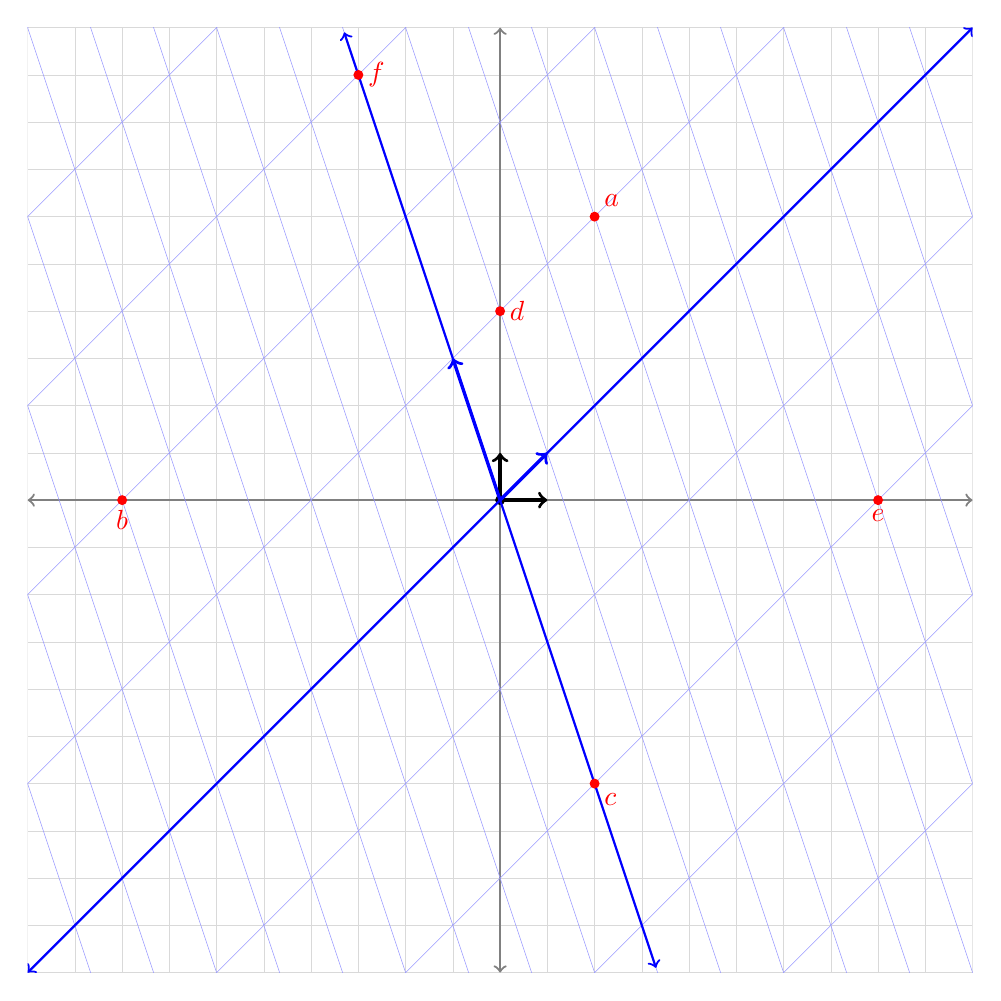
\begin{tikzpicture}[scale=0.6]
    % CLIP EVERYTHING
    \clip(-10,-10)rectangle(10,10);

    % STANDARD COORD SYSTEM
    \draw[gray!30, very thin, step=1] (-10,-10) grid (10,10);
    \draw[gray, thick, <->] (-10,0) -- (10,0);
    \draw[gray, thick, <->] (0,-10) -- (0,10);
    \draw[black, very thick, ->] (0,0) -- (1,0);
    \draw[black, very thick, ->] (0,0) -- (0,1);
    \fill[black] (0,0) circle (3pt);

    % DIFFERENT COORD SYSTEM
    \foreach \k in {-20,...,20} {
    \coordinate (start) at (-10-\k,-10+\k*3);
    \coordinate (end) at (10-\k,10+\k*3);
    \draw[blue!40, very thin] (start) -- (end);
    }
    \foreach \k in {-20,...,20} {
    \coordinate (start) at (-10+\k*1,30+\k*1);
    \coordinate (end) at (10+\k*1,-30+\k*1);
    \draw[blue!40, very thin] (start) -- (end);
    }
    \draw[blue, thick, <->] (-10,-10) -- (10,10);
    \draw[blue, thick, <->] (3.3*1,-3.3*3) -- (-3.3*1,3.3*3);
    \draw[blue, very thick, ->] (0,0) -- (1,1);
    \draw[blue, very thick, ->] (0,0) -- (-1,3);
    
    % RED POINTS
    \fill[red] (2,6) circle (3pt) node[red,above right] {$a$};
    \fill[red] (-8,0) circle (3pt) node[red,below] {$b$};
    \fill[red] (2,-6) circle (3pt) node[red,below right] {$c$};
    \fill[red] (0,4) circle (3pt) node[red,right] {$d$};
    \fill[red] (8,0) circle (3pt) node[red,below] {$e$};
    \fill[red] (-3,9) circle (3pt) node[red, right] {$f$};
    
\end{tikzpicture}
\end{image}

\subsection*{Vragen}

\begin{exercise}
Schrijf de coördinaten van elk van de bovenstaande punten ten opzichte van zowel het blauwe als het zwarte coördinatenstelsel.
\end{exercise}

\begin{exercise}
Bepaal een matrix die:
\begin{enumerate}
\item coördinaten ten opzichte van het blauwe coördinatenstelsel omzet naar coördinaten in het zwarte coördinatenstelsel.
\item coördinaten ten opzichte van het zwarte coördinatenstelsel omzet naar coördinaten in het blauwe coördinatenstelsel.
\end{enumerate}
\begin{hint}
Als je een coördinaat \(\color{blue}\begin{pmatrix} 2 & 1\end{pmatrix}\) in het blauwe coördinatenstelsel gekregen hebt, dan betekent dat in het zwarte coördinatenstelsel:
\[
2\cdot \begin{pmatrix} 1 \\ 1 \end{pmatrix} + 1 \cdot \begin{pmatrix} -1 \\ 3 \end{pmatrix} = \begin{pmatrix} 1 \\ 5 \end{pmatrix}
\]
\end{hint}
\begin{hint}
De uitdrukking \(2\cdot \begin{pmatrix} 1 \\ 1 \end{pmatrix} + 1 \cdot \begin{pmatrix} -1 \\ 3 \end{pmatrix}\) kan je ook schrijven als:
\[\begin{bmatrix} 1 & -1 \\ 1 & 3 \end{bmatrix} \cdot \begin{pmatrix} 2 \\ 1 \end{pmatrix}\]
\end{hint}
\begin{oplossing}
Om van blauw naar zwart om te zetten, vermenigvuldig je de coördinaten met de matrix \(\begin{bmatrix} 1 & -1 \\ 1 & 3 \end{bmatrix}\).\newline
Om van zwart naar blauw om te zetten, vermenigvuldig je de coördinaten met de inverse van die matrix, namelijk \(\begin{bmatrix} \frac{3}{4} & \frac{1}{4} \\ -\frac{1}{4} & \frac{1}{4} \end{bmatrix}\).
\end{oplossing}
\end{exercise}

\begin{exercise}
    Wat is de meeteenheid van het blauwe coördinatenstelsel? Met andere woorden, als je een coördinaat \(\color{blue}\begin{pmatrix} z \\ w \end{pmatrix}\) hebt, wat is dan de meeteenheid?
    \begin{oplossing}
        Het zwarte coördinatenstelsel gebruikt kilometers als meeteenheid.
        Het blauwe coördinatenstelsel gebruikt een andere meeteenheid, namelijk hoe lang je ieder vervoersmiddel gebruikt.
        De meeteenheid is dus in uren, en \(\color{blue}\begin{pmatrix} z \\ w \end{pmatrix}\) betekent dat je het hoverboard \(z\) uur vooruit gebruikt en het magische tapijt \(w\) uur vooruit.
        De waardes \(z\) en \(w\) kunnen ook negatief zijn, wat betekent dat je het vervoersmiddel achteruit gebruikt.
    \end{oplossing}
\end{exercise}

\begin{exercise}
    Gebruikmakend van de blauwe coördinaten, hoeveel tijd neemt het in totaal in beslag om de volgende route af te leggen: \(a \rightarrow b \rightarrow c\)?
    \begin{oplossing}
        De blauwe coördinaten van de punten zijn:
        \begin{itemize}
            \item \(a: \color{blue}\begin{pmatrix} 3 \\ 1 \end{pmatrix}\)
            \item \(b: \color{blue}\begin{pmatrix} -6 \\ 2 \end{pmatrix}\)
            \item \(c: \color{blue}\begin{pmatrix} 0 \\ -2 \end{pmatrix}\)
        \end{itemize}
        De verplaatsing van \(a\) naar \(b\) is dus:
        \[\color{blue}\begin{pmatrix} -6 \\ 2 \end{pmatrix} - \begin{pmatrix} 3 \\ 1 \end{pmatrix} = \begin{pmatrix} -9 \\ 1 \end{pmatrix}\]
        Dit betekent dat je 9 uur achteruit op het hoverboard moet en 1 uur vooruit op het magische tapijt.
        De verplaatsing van \(b\) naar \(c\) is:
        \[\color{blue}\begin{pmatrix} 0 \\ -2 \end{pmatrix} - \begin{pmatrix} -6 \\ 2 \end{pmatrix} = \begin{pmatrix} 6 \\ -4 \end{pmatrix}\]
        Dit betekent dat je 6 uur vooruit op het hoverboard moet en 4 uur achteruit op het magische tapijt.
        Alles samengenomen duurt de route 20 uur.
    \end{oplossing}
\end{exercise}
\end{document}